\documentclass[10pt]{article}

\usepackage{spheric}
%%%TITLE
\title{Simulating shock waves with corrective smoothed particle method (CSPM)}
\date{}

%%AFFILIATIONS
\author[1]{Chunying HUANG$^\dagger$}
\author[1]{Jie DENG}
\author[2]{Darcy Q.HOU}
\author[3]{Arris S. TIJSSELING}

\affil[1]{School of Computer Software, Tianjin University, China}
\affil[2]{School of Computer Science and Technology, Tianjin University, China}
\affil[3]{ Department of Mathematics and Computer Science, Eindhoven University of Technology, The Netherlands}


\affil[$\relax$]{\email{\dagger}{cyhuang416@163.com}}


%%DOCUMENT
\begin{document}

\maketitle

%\SelectedTopics{}

%%PLEASE PUT YOUR ABSTRACT HERE
\begin{abstract}
Numerically solving the compressible Euler equations plays a vital role in many science and engineering problems, among which the shock wave is one of the benchmark tests providing a valuable evaluation for numerical methods. To identify prototypical meshless particle methods for simulating shock waves, the current state-of-the-art Smoothed Particle Hydrodynamics (SPH) schemes with kernel corrections are reviewed.

Among others, the corrective smoothed particle method (CSPM) is an early version of the traditional SPH with corrected kernel and has achieved many successes in both solid \cite{chen1999corrective,chen2001corrective} and fluid dynamics problems \cite{fang2009improved}. It solves the boundary deficiency and tensile instability problems in traditional SPH. The meshless finite particle method (FPM) of Liu et al. \cite{liu2005modeling} shares the same merit as CSPM. However, as shown in the well-known textbook on SPH \cite{liu2003smoothed}, CSPM failed to capture the shock physics (see Figs. 5.7-5.10 in \cite{liu2003smoothed}). Based on Taylor series expansion borrowed from CSPM, Liu and Liu \cite{liu2003smoothed} developed a discontinuous SPH (DSPH) for shock waves. However, an effective discontinuity detection algorithm has to be used, which can be rather challenging in multi-dimensional problems. In this paper, together with the SPH summation form of the continuity equation, the CSPM is applied to simulate shock waves and good results were obtained as shown in Fig. \ref{fig:50}. To enhance the performance, a variable smoothing length was also employed, together with virtual particle method for boundaries.

\begin{figure}[!htb]
\centering
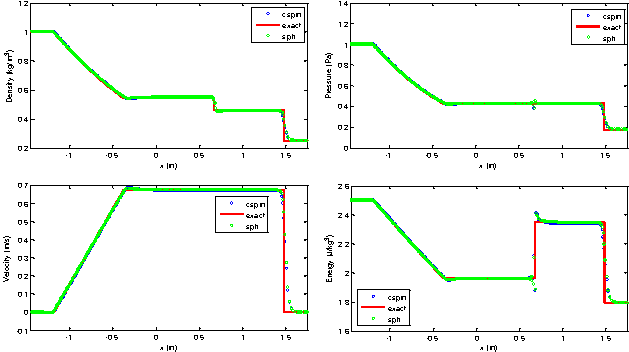
\includegraphics[width=0.75\textwidth]{50-1.pdf}
\caption{Numerical results for the shock tube problem obtained with different versions of SPH formulation.}\label{fig:50}
\end{figure}

\end{abstract}


%%THE END OF ABSTRACT

\addbib

\end{document}
